\section{Attitude Control of Satellite}
\subsection{}
\subsubsection{Finding equilibrium}
We are given the following equations of motion (EoM) for the satellite
\begin{equation}
\label{eq:dynamics}
	\begin{aligned}
		\dot{\mathbf{q}} = \mathbf{T}_q (\mathbf{q} ) \boldsymbol{\omega}, \\
		\mathbf{I}_{CG} \dot{\boldsymbol{\omega}} - \mathbf{S} (\mathbf{I}_{CG} \boldsymbol{\omega} ) \boldsymbol{\omega} & =  \boldsymbol{\tau}.
	\end{aligned}
\end{equation}
To linearize this, we must first find an equilibrium point. We set the derivatives $\dot{\mathbf{q}}$ and $\dot{\boldsymbol{\omega}}$ equal to zero and in addition require $\mathbf{q} = [\eta, \epsilon_1, \epsilon_2, \epsilon_3]^\top  = [\eta, 0, 0, 0]^\top$ and $\boldsymbol{\tau} = \mathbf{0}$ thus obtaining
\begin{align}
\label{eq:ang_vel_trans_1}
\mathbf{T_q}(\mathbf{q})\boldsymbol{\omega}_0 = \mathbf{0}, \\
\label{eq:ang_vel_trans_2}
\mathbf{S}(\mathbf{I}_{CG} \boldsymbol{\omega}_0)\boldsymbol{\omega}_0 = \mathbf{0}.
\end{align}
Using (2.69) from \cite{Fossen2011} we can rewrite \eqref{eq:ang_vel_trans_1} and obtain
\begin{equation}\begin{aligned}
\mathbf{T_q}(\mathbf{q})\boldsymbol{\omega}_0
&= \frac{1}{2}
\begin{bmatrix}
- \boldsymbol{\epsilon}_0^\top \\
\eta \mathbf{I}_3 + \mathbf{S}(\boldsymbol{\epsilon}_0)
\end{bmatrix}
\boldsymbol{\omega}_0 \\
&= \frac{1}{2}
\begin{bmatrix}
\mathbf{0}^\top \\
\mathbf{I}_3
\end{bmatrix}
\boldsymbol{\omega}_0 \\
&= \mathbf{0}.
\end{aligned}\end{equation}
Hence $\boldsymbol{\omega}_0 = \mathbf{0}^\top$ and we have the equilibrium point $\mathbf{x}_0 = [\boldsymbol{\epsilon}_0^\top, \boldsymbol{\omega}_0^\top]^\top = \mathbf{0}^\top$. This clearly also satisfies \eqref{eq:ang_vel_trans_2}.
\subsubsection{Linearizing around equilibrium}
We wish to linearize this non-linear system around $\mathbf{x}_0$. For that, we need expressions for $\dot{\boldsymbol{\epsilon}}$ and $\dot{\boldsymbol{\omega}}$. We find
\begin{align}
\dot{\boldsymbol{\epsilon}}
&= \frac{1}{2}(\eta \mathbf{I}_3 + \mathbf{S}(\boldsymbol{\epsilon}))\boldsymbol{\omega}
= \frac{1}{2}\eta \boldsymbol{\omega} + \frac{1}{2}\mathbf{S}(\boldsymbol{\omega})\boldsymbol{\omega}
= \frac{1}{2}\eta \boldsymbol{\omega}
= \frac{1}{2}\sqrt{1 - \boldsymbol{\epsilon}^\top\boldsymbol{\epsilon}}\boldsymbol{\omega}, \quad \text{and} \\
\dot{\boldsymbol{\omega}}
&= \mathbf{I}_{CG}^{-1}(\mathbf{S}(\mathbf{I}_{CG}\boldsymbol{\omega})\boldsymbol{\omega} + \boldsymbol{\tau})
=\frac{1}{mr^2}(\mathbf{S}(\mathbf{I}_{CG}\boldsymbol{\omega})\boldsymbol{\omega} + \boldsymbol{\tau})
= \boldsymbol{S}(\boldsymbol{\omega})\boldsymbol{\omega} + \frac{1}{mr^2}\boldsymbol{\tau}
= \frac{1}{mr^2}\boldsymbol{\tau}.
\end{align}
So,
\begin{equation}\begin{aligned}
\dot{\mathbf{x}} =
\begin{bmatrix}
\dot{\boldsymbol{\epsilon}}\\
\dot{\boldsymbol{\omega}}\\
\end{bmatrix}
=\begin{bmatrix}
\frac{1}{2}\sqrt{1-\boldsymbol{\epsilon}^\top\boldsymbol{\epsilon}}\boldsymbol{\omega}\\
\frac{1}{mr^2}\boldsymbol{\tau}\\
\end{bmatrix}
= \mathbf{f}(\mathbf{x}, \boldsymbol{\tau}).
\end{aligned}\end{equation}
The linearized system has the form
\begin{equation}\begin{aligned}
\dot{\hat{\mathbf{x}}} = \mathbf{A}\hat{\mathbf{x}} = \mathbf{B}\hat{\boldsymbol{\tau}}
\end{aligned}\end{equation}
where $\mathbf{A} = $ and $\mathbf{B}$ are the Jacobians $\frac{\partial \mathbf{f}}{\partial \mathbf{x}}$, and $\frac{\partial \mathbf{f}}{\partial \boldsymbol{\tau}}$ respectively, evaluated at the equilibrium $\mathbf{x}=\mathbf{x_0}$. That is,
\begin{align}
\label{eq:A_matrix}
\mathbf{A}
&= \begin{bmatrix}
-\frac{1}{2}\sqrt{1-\boldsymbol{\epsilon}_0^\top\boldsymbol{\epsilon}_0}\boldsymbol{\epsilon}_0\boldsymbol{\omega}_0^\top & \frac{1}{2}\sqrt{1-\boldsymbol{\epsilon}_0^\top\boldsymbol{\epsilon}_0}\mathbf{I}_3\\
\mathbf{0}_3 & \mathbf{0}_3 \\
\end{bmatrix}
= \begin{bmatrix}
\mathbf{0}_3 & \frac{1}{2}\mathbf{I}_3 \\
\mathbf{0}_3 & \mathbf{0}_3 \\
\end{bmatrix}, \quad \text{and} \\
\mathbf{B}
\label{eq:B_matrix}
&= \begin{bmatrix}
\mathbf{0}_3\\
\frac{1}{mr^2}\mathbf{I}_3\\
\end{bmatrix}
\end{align}
where $\mathbf{0}_3$ denotes a 3-by-3 zero-valued matrix. \eqref{eq:A_matrix} follows from the following results
\begin{align}
\frac{\partial}{\partial \epsilon_i}\frac{1}{2}\sqrt{1-\epsilon_1^2 - \epsilon_2^2 - \epsilon_3^2}\omega_k
&= -\frac{1}{2}\sqrt{1-\epsilon_1^2 - \epsilon_2^2 - \epsilon_3^2}^{-1}\epsilon_i \omega_k, \\
\frac{\partial}{\partial \omega_i}\frac{1}{2}\sqrt{1-\boldsymbol{\epsilon}^\top\boldsymbol{\epsilon}}\omega_i
&=\frac{1}{2}\sqrt{1-\boldsymbol{\epsilon}^\top\boldsymbol{\epsilon}}.
\end{align}


\subsection{}

\subsection{}
Equation (2) from the assignment can be written as:
\begin{equation}
  \label{eq:tau}
  \mathbf{\tau} = -\mathbf{K}_d \boldsymbol{\omega} - k_p \boldsymbol{\epsilon}
\end{equation}

\subsection{}
The quaternion error can be written as
 \begin{equation}
	 \tilde{\mathbf{q}} := \left[
	 \begin{array}{c}
		 \tilde{\eta} \\
		 \tilde{\epsilon}
	 \end{array}
	 \right] = \bar{\mathbf{q}}_d \otimes \mathbf{q}
 \end{equation}

\subsection{Problem 1.5}
In problems with simulations, you need to include figures in the report:
\begin{figure}[ht]
	\centering
	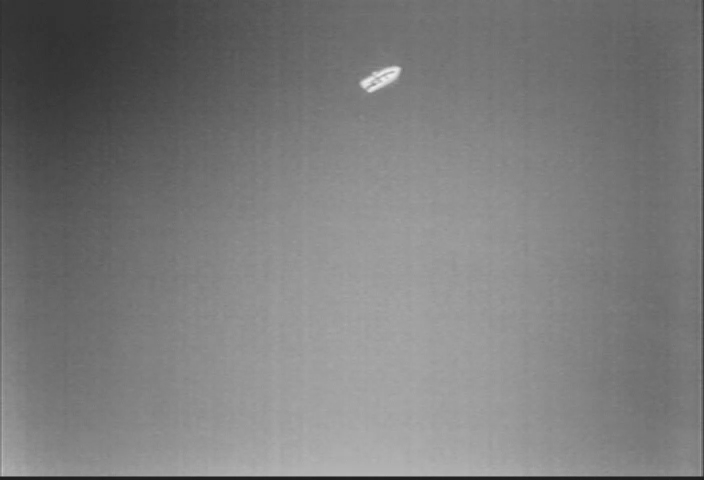
\includegraphics[width=0.7\textwidth]{fig1} % Filename is "fig1.png" and must be located in the same folder as this file. If you have a folder containing all the figures you can use "Figures/fig 1" as long as the "Figures" folder is placed in the same folder as this file.
	\caption{Figure of something useful.}
	\label{fig:fig1}
\end{figure}

You can now refer to this figure as \figref{fig:fig1}. You can also insert figures side-by-side as in Figure \ref{fig:2}. %Notice that \figref includes the word Figure before the reference. If you use "\ref", you need to write the word Figure yourself.
\begin{figure}[ht]
	\centering
	\begin{subfigure}[b]{0.45\textwidth}
		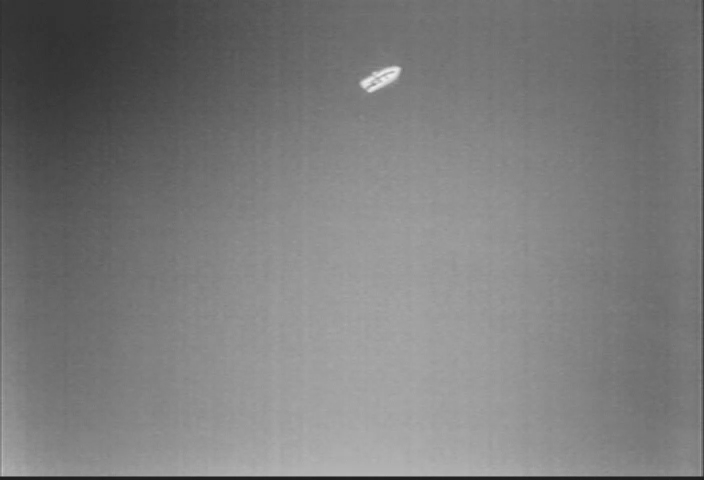
\includegraphics[width=\textwidth]{fig1}
		\caption{caption..}
		\label{fig:2a}
	\end{subfigure}
	~ %add desired spacing between images, e. g. ~, \quad, \qquad, \hfill etc.
	%(or a blank line to force the subfigure onto a new line)
	\begin{subfigure}[b]{0.45\textwidth}
		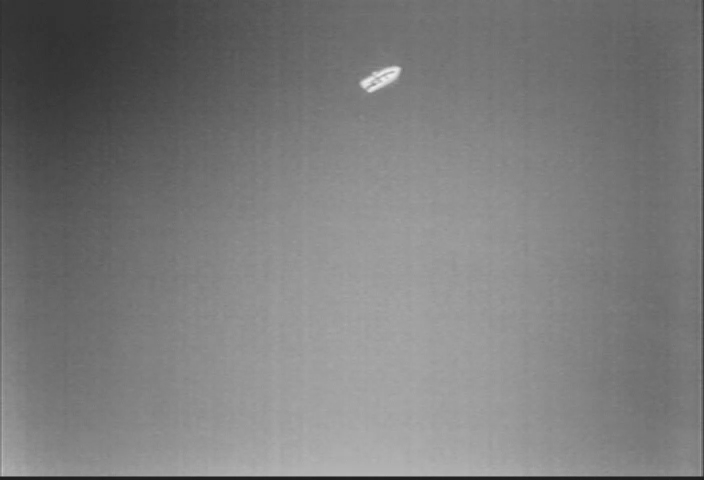
\includegraphics[width=\textwidth]{fig1}
		\caption{caption..}
		\label{fig:2b}
	\end{subfigure}
	\begin{subfigure}[b]{0.45\textwidth}
		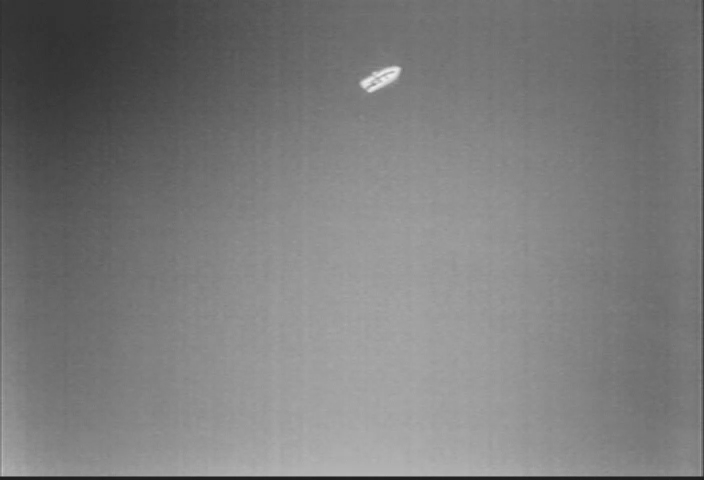
\includegraphics[width=\textwidth]{fig1}
		\caption{caption..}
		\label{fig:2c}
	\end{subfigure}
	\begin{subfigure}[b]{0.45\textwidth}
		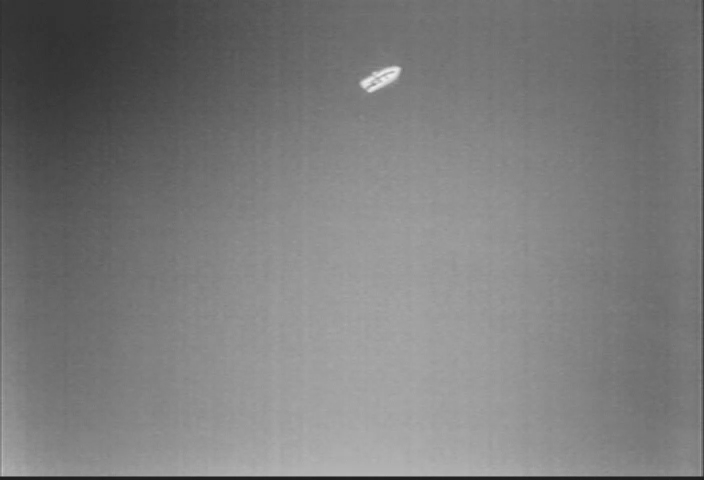
\includegraphics[width=\textwidth]{fig1}
		\caption{caption..}
		\label{fig:2d}
	\end{subfigure}
	\caption{Caption for all figures}\label{fig:2}
\end{figure}


\subsection{Problem 1.6}
The control law in this problem can be written as
\begin{equation}
	\boldsymbol{\tau} = -\mathbf{K}_d \tilde{\boldsymbol{\omega}} - k_p \tilde{\boldsymbol{\epsilon}}
\end{equation}
and the desired angular velocity as
\begin{equation}
	\boldsymbol{\omega}_d = \mathbf{T}^{-1}_{\Theta_d}(\Theta_d)\dot{\Theta}_d
\end{equation}

\subsection{Problem 1.7}
The Lyapunov function can be written as
 \begin{equation}
	 V = \frac{1}{2} \tilde{\boldsymbol{\omega}}^{\top} \mathbf{I}_{CG}\tilde{\boldsymbol{\omega}} + 2 k_p (1-\tilde{\eta})
 \end{equation}
and the derivative as
\begin{equation}
	\dot{V} = -k_d \boldsymbol{\omega}^{\top} \boldsymbol{\omega}
\end{equation}

% Note that \mathbf can be used for bold letters in math mode (within equations and dollar signs). \boldsymbol can be used to get bold greek letters.
